\documentclass[lang=cn,a4paper]{elegantpaper}

\title{数学建模}
\author{作者:陶理}
\institute{中三(2)班 28号 \\  上海市实验学校}
\date{\zhtoday}

\usepackage{url,appendix,graphicx,float,multicol}
\usepackage[version=4]{mhchem}
\begin{document}

    \maketitle

    \section{第一题}
    \subsection{问题分析}
    \subsubsection*{分析方式}
    编程:Python语言

    所需第三方库:numpy,matplotlib
    
    将题目所给的x、y数据转化为python中的list数据类型(即数组),通过plotfit函数进行多项式拟合。
    \subsubsection*{判断耦合程度}
    思路来源:方差和标准差
    $$
    s^2=\frac{1}{n}\sum_{i=1}^n (a_i-\bar{a})^2,s=\sqrt{\frac{1}{n}\sum_{i=1}^n (a_i-\bar{a})^2}~~~~~~~~~~~~(\bar{a}=\frac{1}{n}\sum_{i=1}^n a_i)
    $$

    记原本的数值是$x_i$对应$y_i(1\leqslant x\leqslant n,x\in \mathbb{Z}^+)$

    记拟合函数为$f(x)$,使用拟合函数预测的数值为$p_i=f(a_i)~~(1\leqslant x\leqslant n,x\in \mathbb{Z}^+)$
    
    通过$p_i$和$b_i$之间的误差可以判断拟合函数f(x)和原曲线的耦合程度,误差越小说明耦合程度越好。
    $$
    \Delta^2=\frac{1}{n}\sum_{i=1}^n (p_i-b_i)^2, \Delta=\sqrt{\frac{1}{n}\sum_{i=1}^n (p_i-b_i)^2}
    $$
    \subsection{拟合结果}
    三次:$y=3.734x^3-150.8x^2+1251x-2447$

    $\Delta_3=1122.1100$
    \begin{figure}[H]
        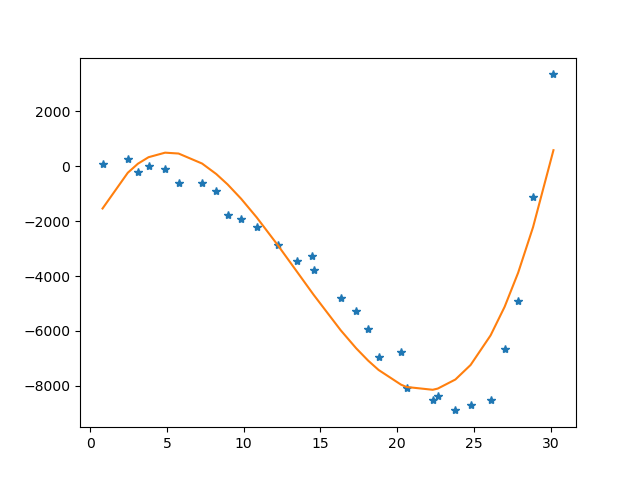
\includegraphics[scale=0.4]{1-3.png}
    \end{figure}
    四次:$y=0.2556x^4-12.13x^3+169.2x^2-1041x+1633$

    $\Delta_4=502.2787$
    \begin{figure}[H]
        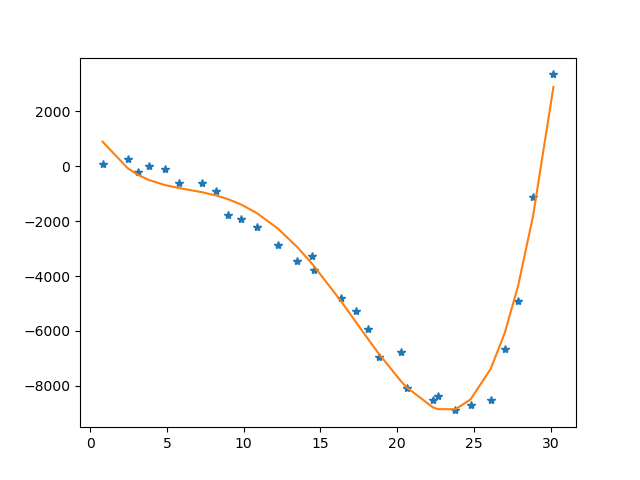
\includegraphics[scale=0.4]{1-4.png}
    \end{figure}
    五次:$y=0.01262x^5-0.7224x^4+15.01x^3-152.9x^2-464.9x-236.6$

    $\Delta_5=322.8720$
    \begin{figure}[H]
        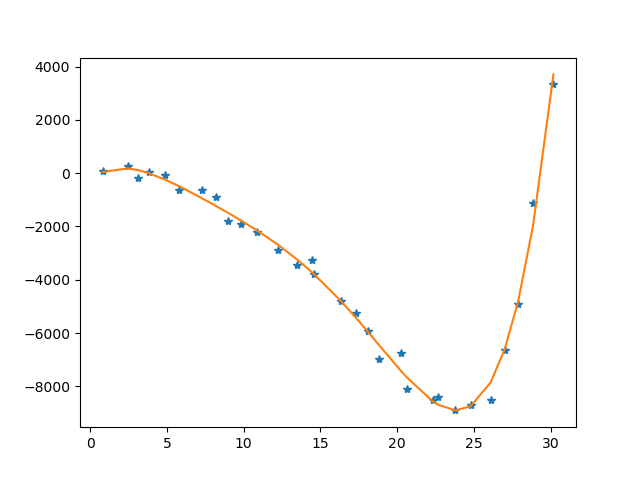
\includegraphics[scale=0.4]{1-5.png}
    \end{figure}
    六次:$y=-5.661\times 10^{-5} x^6+0.01787x^5-0.9075x^4+18.09x^3-177.4x^2+545.3x-309.3$

    $\Delta_6=319.3721$
    \begin{figure}[H]
        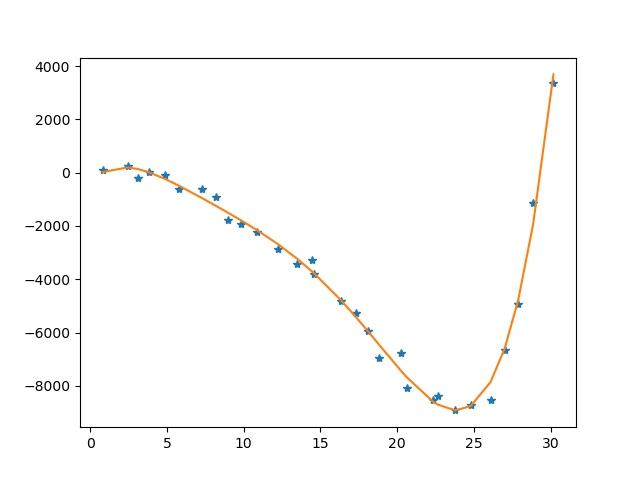
\includegraphics[scale=0.4]{1-6.png}
    \end{figure}
    \clearpage
    七次:$y=-5.622\times10^{-5}x^7+0.006036x^6-0.2443x^5+4.778x^4-47.04x^3+198.1x^2-382x+331.3$

    $\Delta_7=498.2919$
    \begin{figure}[H]
        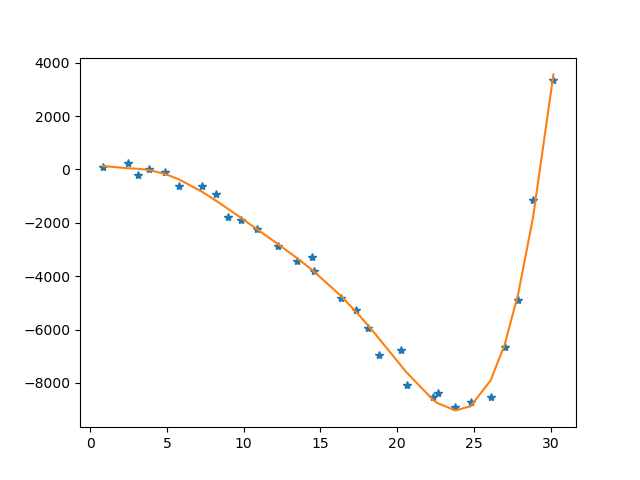
\includegraphics[scale=0.4]{1-7.png}
    \end{figure}
    \subsection{对比分析}
    误差排序:$\Delta_6<\Delta_5<\Delta_7<\Delta_4<\Delta_3$
    在所记录的5个不同次数的多项式中,六次多项式和五次多项式的拟合效果较好,因为误差较小。

    \clearpage

    \section{第二题}
    \subsection{问题分析}
    \subsubsection*{题目:}
    小旭家现有1千克馄饨/饺子馅,小旭准备自己动手包一些馄饨/饺子,他想知道需要准备多少馄饨/饺子皮。试建立数学模型,讨论对于肉馅或菜肉馅、对于方形的馄饨皮或圆形的饺子皮,1千克馅料分别需要多少面皮可以恰好把所有馅料做成馄饨/饺子?
    \subsubsection*{条件:}
    \begin{itemize}
        \item 有1kg的馄饨/饺子馅
        \item 馄饨皮是方的,饺子皮是圆的
        \item 馅有两种选择:肉馅或菜肉馅
    \end{itemize}
    \subsubsection*{分析:}
    问1kg馅料分别需要多少面皮可以恰好把所有馅料做成馄饨/饺子,其实可以等效看作1kg的馅料可以包多少馄饨/饺子。而这个问题可以最终看作一个饺子能包多少质量的馅料,即一张面皮对应的馅料的质量。

    根据化简后问题“一张面皮对应的馅料的质量”以及物理公式$m=\rho V$,需要知道馅料的密度以及一张面皮中能放多少体积的馅料。而一张面皮中能放多少体积的馅料取决于面皮的大小,所以需要设定面皮的边长或者直径(或半径)。
    \subsection{建立模型}
    将馅料看作一个长径为$r_1~cm$,两条短径相同均为$r_2~cm$的椭球体(如下图所示)。
    \begin{figure}[H]
        \centering
        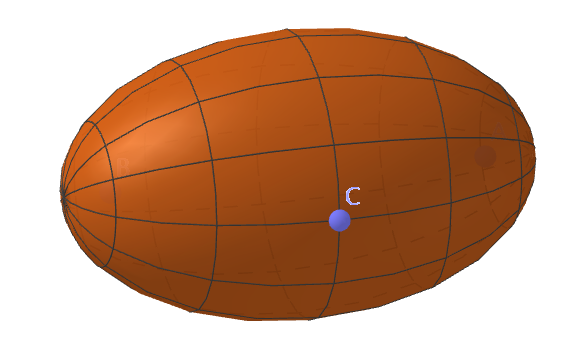
\includegraphics[scale=0.2]{ellipsoids.png}
    \end{figure}
    将馄饨皮近似看成以$a~cm$为边长的正方形(如图所示)
    \begin{figure}[H]
        \centering
        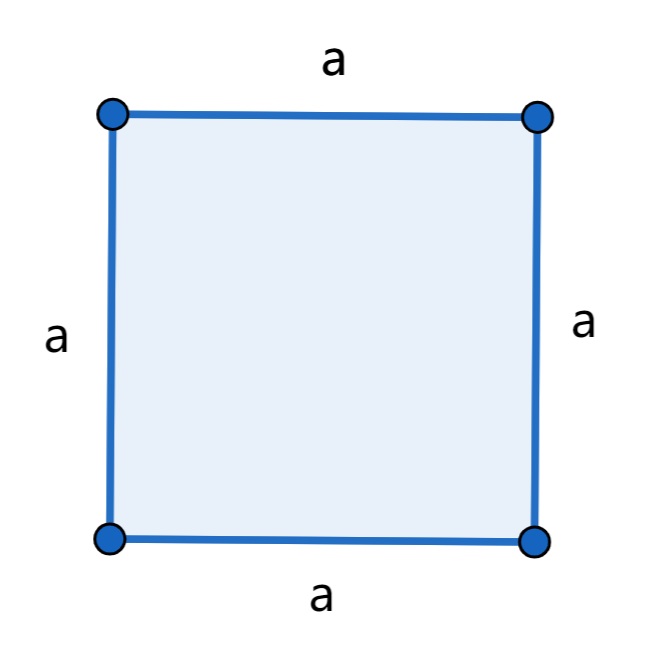
\includegraphics[scale=0.5]{square.png}
    \end{figure}
    将饺子皮近似看成以$a~cm$为半径的圆
    \begin{figure}[H]
        \centering
        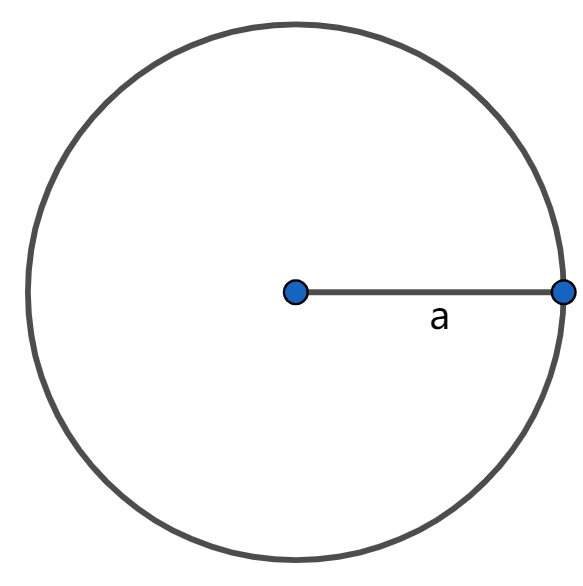
\includegraphics[scale=0.4]{circle.png}
    \end{figure}
    需要考虑到饺子/馄饨皮并不是完全用于包裹馅料,还需要有部分用来粘合和包外层的褶皱。对于饺子皮而言,可以看作有一圈周围的圆环用于粘合,实际包裹馅料的面积应减掉圆环部分。通过观察,周围褶皱部分宽度$w~cm$大概为半径的$\dfrac{1}{3}$到$\dfrac{1}{2}$左右,此处折中考虑,即为$w=\dfrac{\frac{1}{3}+\frac{1}{2}}{2}a=\dfrac{5}{12}a~cm$
    \begin{figure}[H]
        \centering
        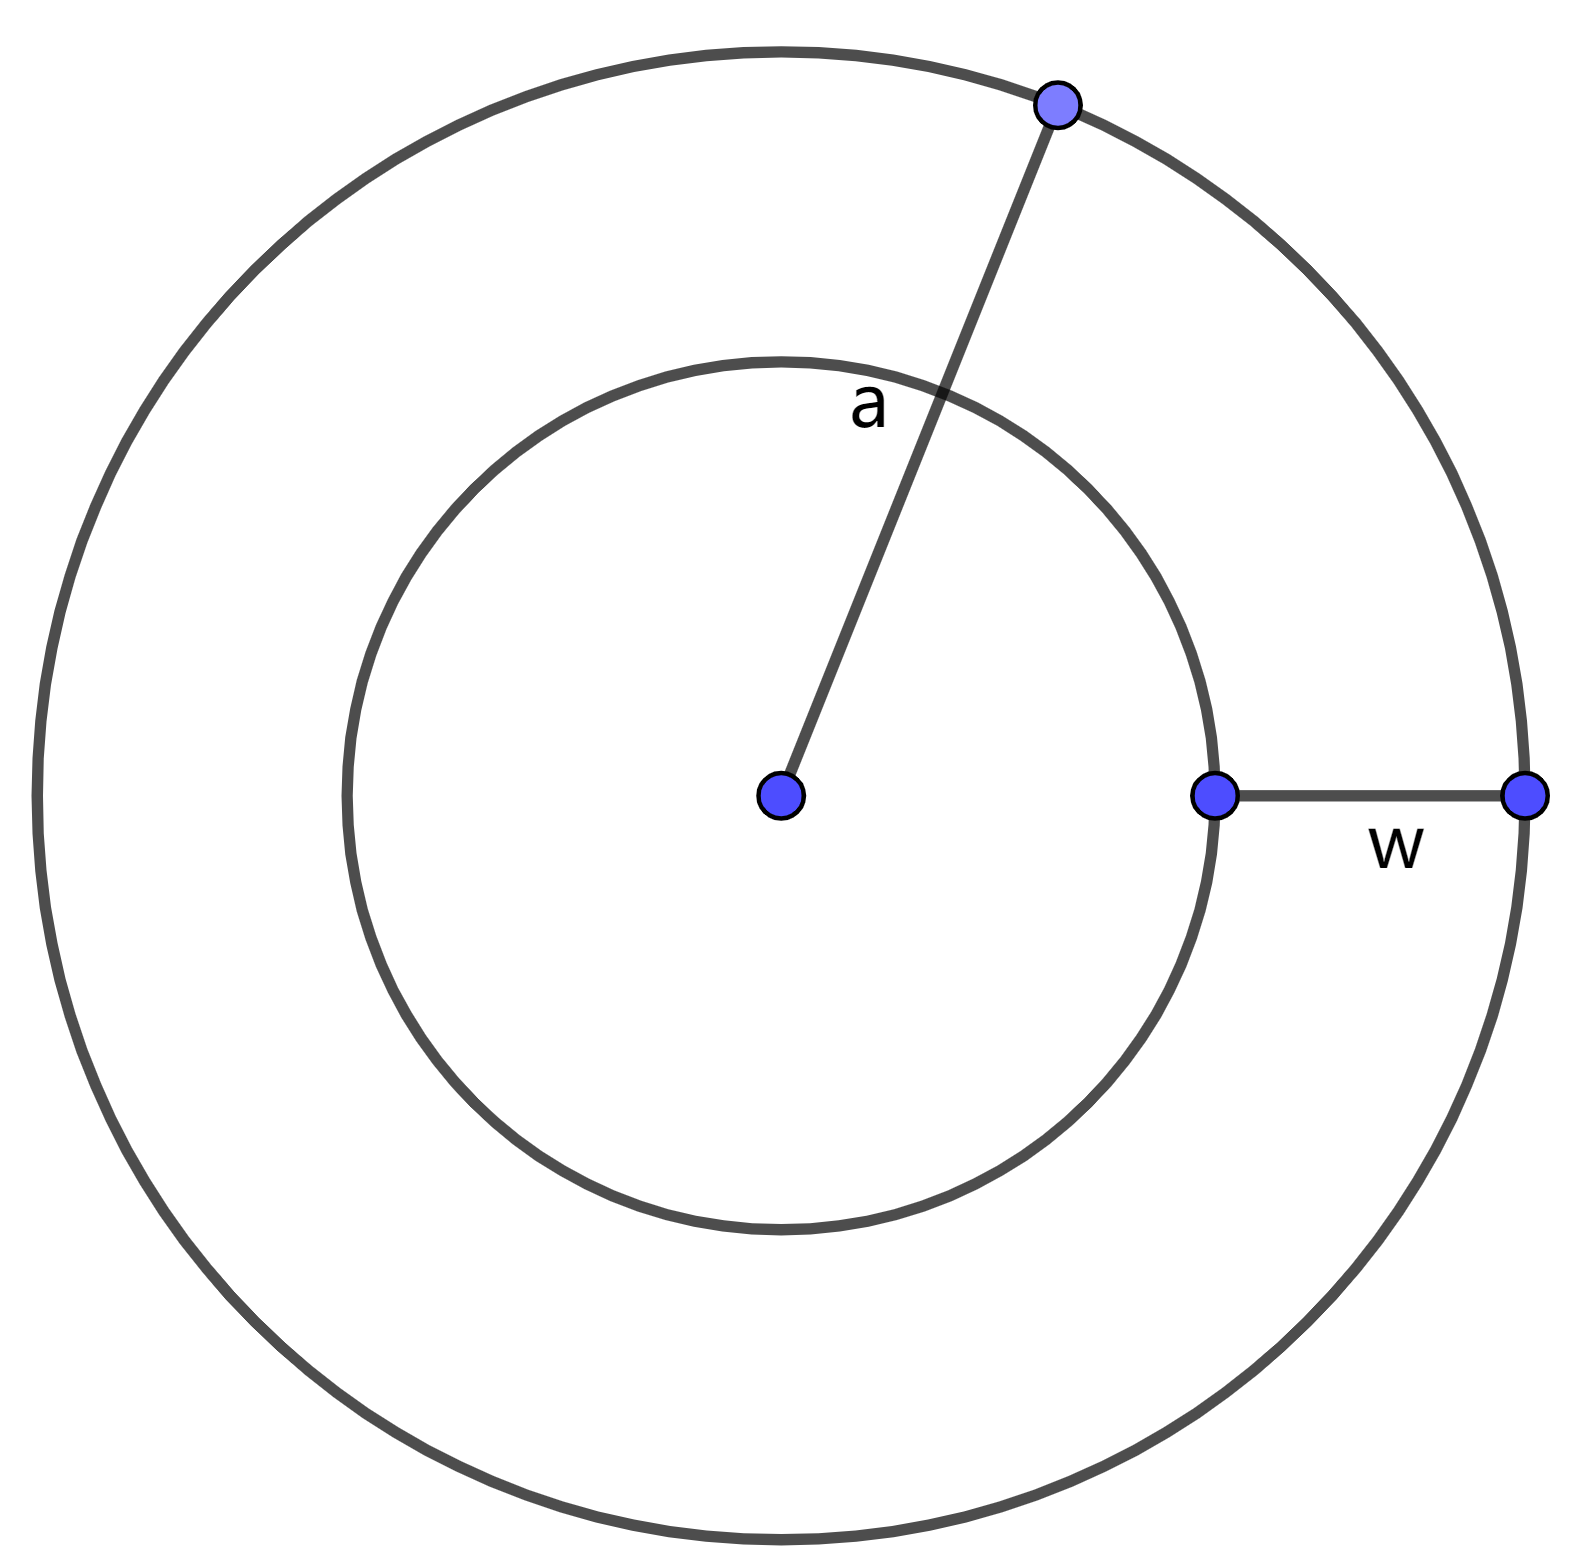
\includegraphics[scale=0.25]{circle_1.png}
    \end{figure}
    
    则馅料椭球体的长径$r_1$约为$a-w=\dfrac{7}{12}a~cm$,两条短径相等,$r_2$约为$\dfrac{r_1}{2}=\dfrac{a-w}{2}=\dfrac{\dfrac{7}{12}a}{2}=\dfrac{7}{24}a~cm$,根据椭球体体积公式:$V=\dfrac{4}{3}\pi abc$,则馅料的体积约为$V_{fill}=\dfrac{4}{3}\pi r_1r_2^2=\dfrac{4}{3}\pi \cdot \dfrac{7}{12}a \cdot (\dfrac{7}{24}a)^2=\dfrac{343}{5184}\pi a^3~cm^3$

    经调查,$\rho_{fat}=0.74g/cm^3,\rho_{muscle}=1.12g/cm^3$
    
    一般做馄饨/饺子的肉馅中肥肉(主体为脂肪)和瘦肉(主体为肌肉)的比例约为3:7,所以$\rho_{fill}=\dfrac{3\rho_{fat}+7\rho_{muscle}}{10}=1.006g/cm^3$。又饺子馅中需要加酱油等调料和水,所以将馅料的密度近似看为水的密度,方便计算,即$\rho_{fill}\approx\rho_{\ce{H2O}}=1g/cm^3$

    所以$m_{fill}=p_{fill}V_{fill}=1g/cm^3 \cdot \dfrac{343}{5184}\pi a^3~cm^3=\dfrac{343}{5184}\pi a^3~g$

    所以$num_{Wonton}=\lfloor 1kg/m_{fill} \rfloor=\lfloor \dfrac{5184000}{343\pi a^3}\rfloor$
    \clearpage
    \section{第三题}
    \subsection{分析问题}
    \subsubsection*{题目}
    俄罗斯方块是一款家喻户晓的电子游戏,小数对其深感兴趣,将其简化规则如下:
    \begin{itemize}
        \item 游戏中,一共有四种基础方块
        \item 每一轮游戏中,给定的基础方块的种类和数目一定,但摆放方块的先后顺序锁定,不可更改
        \item 游戏提供的“方格容器”宽度为八个单位长度,高度无限每一个基础方块都可以进行自由旋转、翻转
        \item 玩家的最终目的是使用最小的高度完成所有方块的摆放
        \item 得到摆放完整的一行并不可以消除方块,但可以得到额外加分
    \end{itemize}

    1. 根据题目描述,给出一种界定方块摆放有效率的方式(即这个游戏的分数计算方式),并用数学语言进行描述。

    2. 若某一局游戏中,方块下落的顺序已提前知晓如图2所示,试找到赢得这场比赛的最佳策略并用文字语言、数学语言或者图表描述你的策略.并根据你提供的计分方式得出结果。
    \begin{figure}[H]
        \centering
        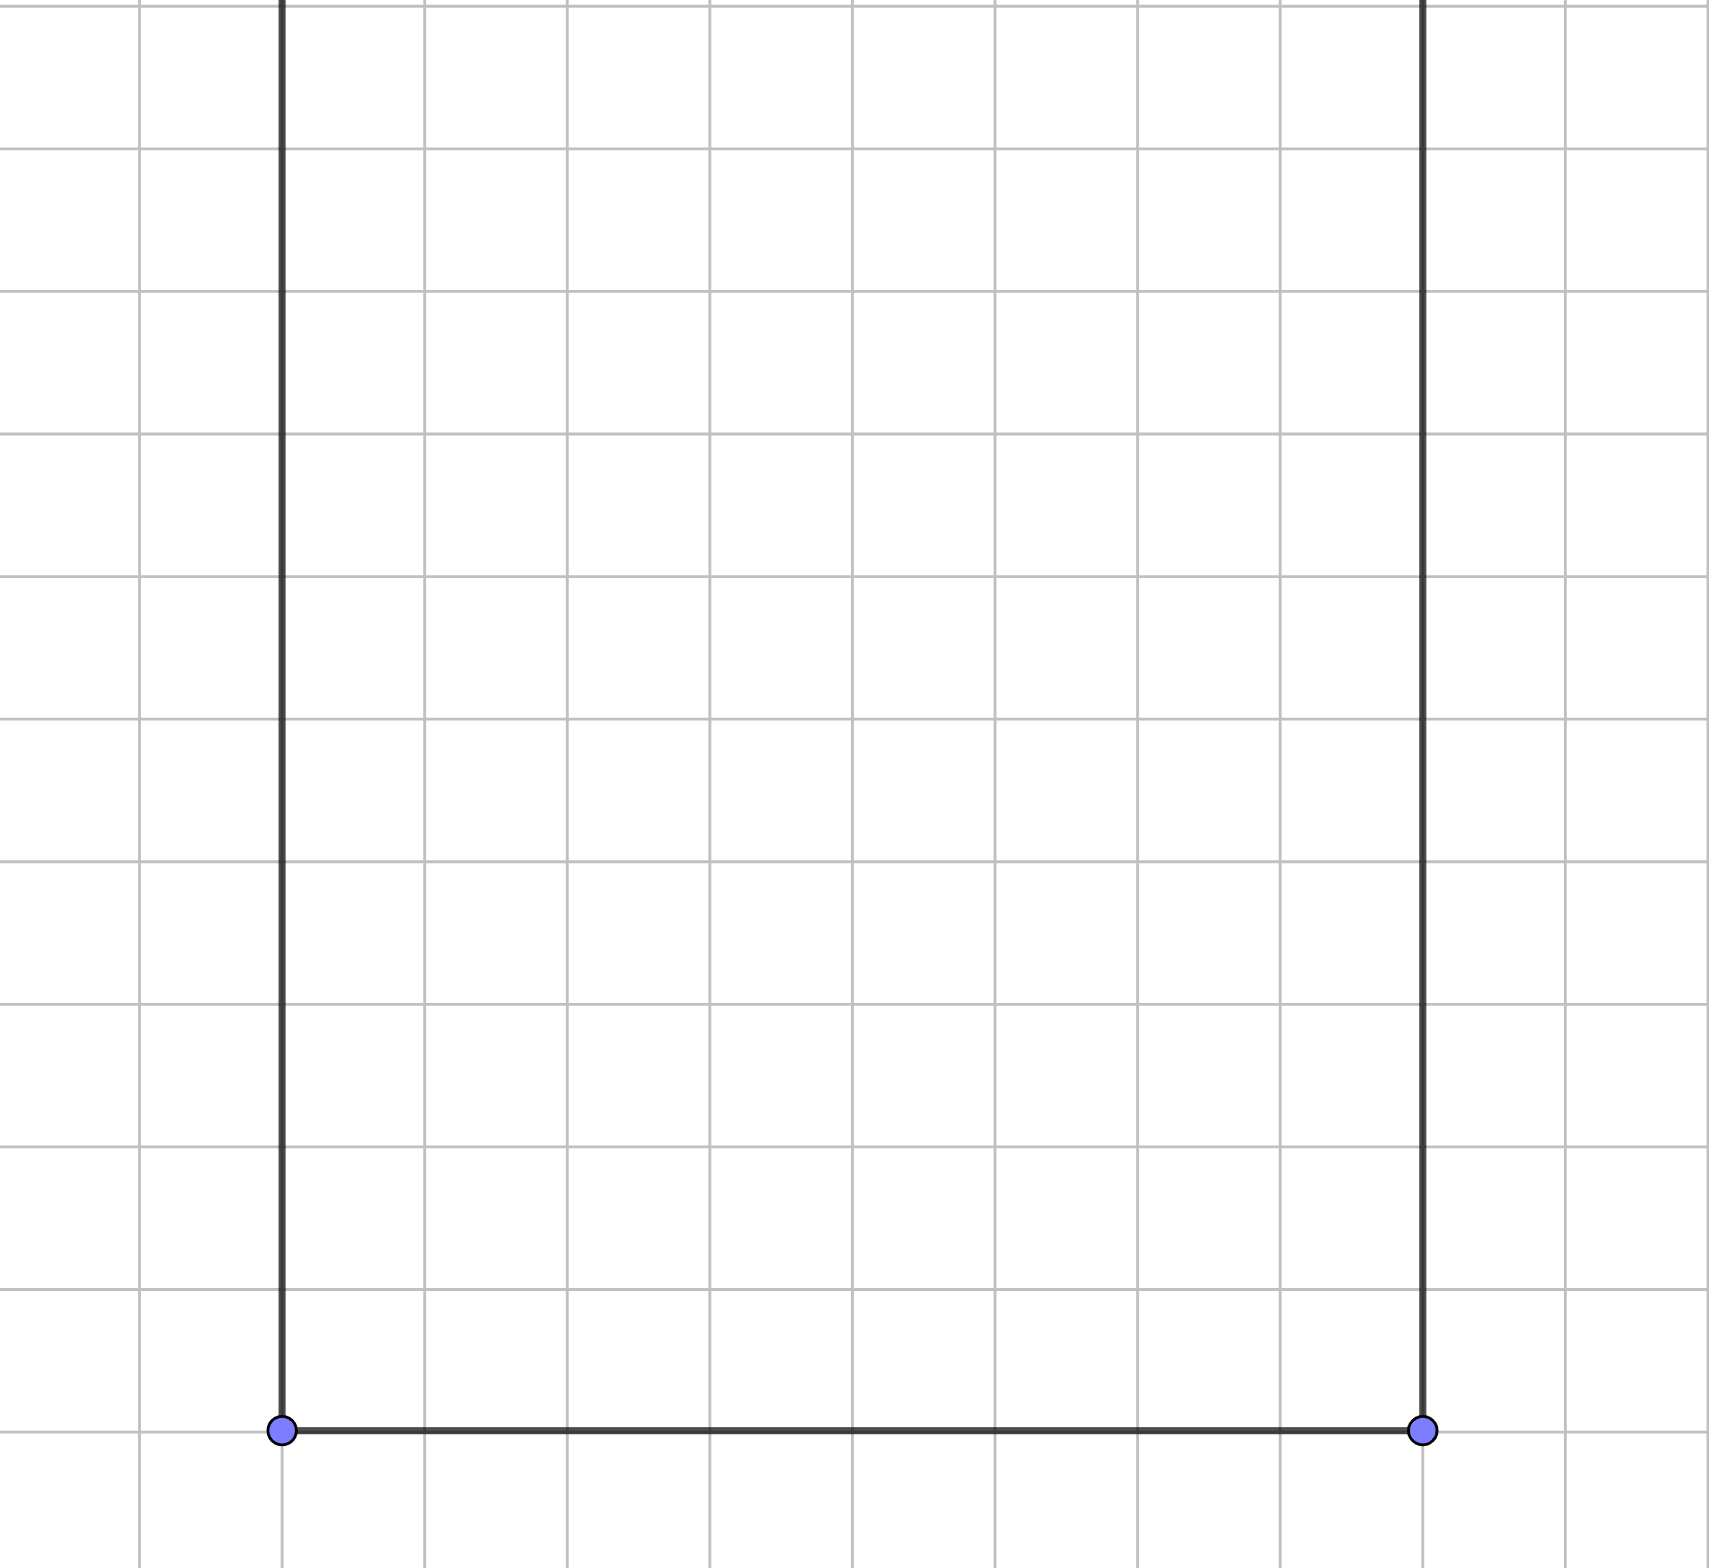
\includegraphics[scale=0.2]{Container.png}
        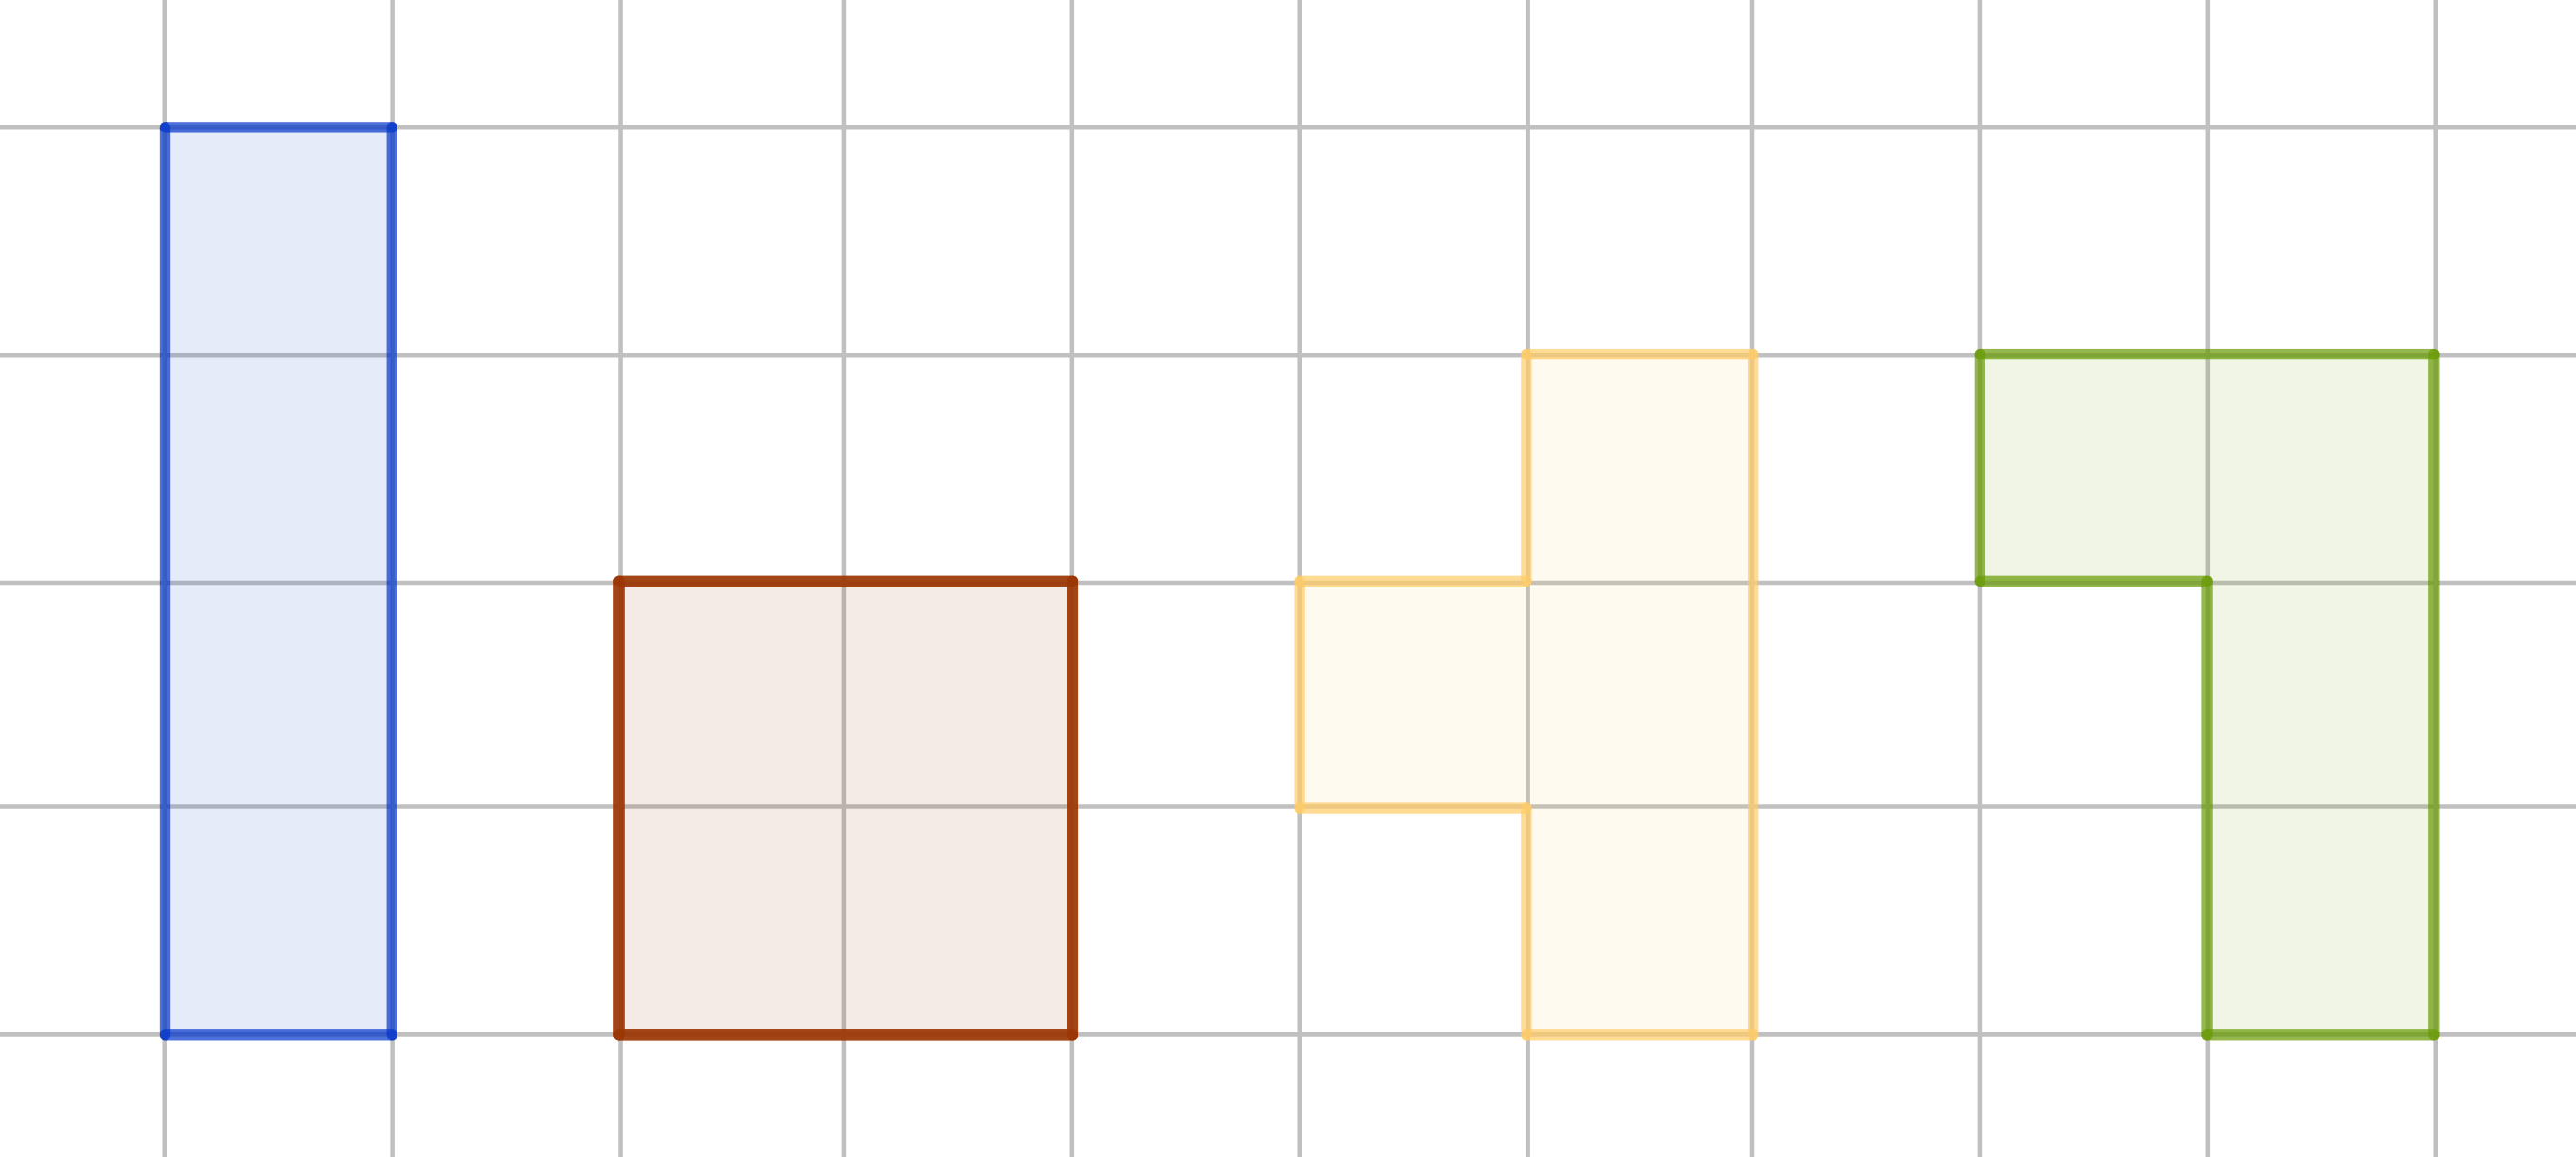
\includegraphics[scale=0.4]{basic units.png}
    \end{figure}
    \subsubsection{第一小问}
    根据“玩家的最终目的是使用最小的高度完成所有方块的摆放”,可以看出,层数越高分数应该越低。根据“得到摆放完整的一行并不可以消除方块,但可以得到额外加分”,可以看出,分数计算方式应该考虑到完整的一行加分。其余条件与分数无关。

    假设分数函数为$F(x)=S(x)+Ex(x)$,其中$S(x)$为高度所对应的分数,$Ex(x)$为摆放完整的行所对应的加分。则$\displaystyle\lim_{x\rightarrow \infty}S(x)=0$

    既然对于每一局,给定的基础方块的种类和数目一定,所以覆盖的总面积应该是已知的。将基础方块进行编号,“$1\times4$”的蓝色方块标记为1号,“$2\times2$”的橙色方块标记为2号,凸状的黄色方块标记为3号,类似“7”的绿色方块标记为4号。记一共出现i号方块$cnt_i$次$(1\leqslant i\leqslant 4,i\in\mathbb{Z})$,则方块覆盖面积$\displaystyle A=\sum_{i=1}^4 4cnt_i=4\sum_{i=1}^4 cnt_i$。
    
    摆放的理论最大高度为$\displaystyle H_{max}=4cnt_1+2cnt_2+3cnt_3+3cnt_4=cnt_1-cnt_2+3\sum_{i=1}^4{cnt_i}. $因为“方格容器”宽度为8个单位长度,所以摆放的理论最小高度为$\displaystyle H_{min}=\lceil \dfrac{A}{8} \rceil=\lceil \frac{1}{2}\sum_{i=1}^4 cnt_i \rceil.$所以摆放的高度范围为:$\displaystyle \lceil \dfrac{1}{2} \sum_{i=1}^4 cnt_i\rceil \leqslant H \leqslant cnt_1-cnt_2+3\sum_{i=1}^4{cnt_i}$

    设摆放的实际最小高度为${H\_F}_{min}$,则${H\_F}_{min}\geqslant H_{max}$
\end{document}